\section{Two coupled pendulums}
\label{sec:coupled}

We take
\begin{equation}
V(q_1,q_2) = -\cos q_1 - \cos q_2 - \varepsilon\cos(q_1 - q_2), \qquad \varepsilon \neq 0 .
\label{eq:coupledV}
\end{equation}

\emph{Maximal strain.} For $\varepsilon > 0$ the maximum is at $q_0 = (\pi, 0)$, where
\begin{equation}
M(q_0) = \frac12\begin{pmatrix} 2+\varepsilon & -\varepsilon \\ -\varepsilon & \varepsilon \end{pmatrix},
\qquad
\kappa(\varepsilon) = \frac{1 + \varepsilon + \sqrt{1+\varepsilon^2}}{2},
\label{eq:coupledkappa}
\end{equation}
with $e_+ \propto \big(\varepsilon,\; 1 - \sqrt{1+\varepsilon^2}\big)$: the first pendulum sits at its unstable top and the second at its bottom, and the most stretching direction is mainly the first pendulum's, tilted slightly into the second. For $\varepsilon < 0$ the maximum moves to $q_0 = (\pi,\pi)$, both pendulums at the top, with $\kappa = 1 - \varepsilon$ and $e_+ = (1,-1)/\sqrt2$: the coupling raises the stretching of the antisymmetric motion. The values at $q_0$ are exact; that they are the suprema over the torus was checked on a $1441^2$ grid. For $\varepsilon = 0$ the maximum is degenerate, $\kappa = 1$ on the lines $q_1 = \pi$ and $q_2 = \pi$, and the assumption of Sec.~\ref{sec:setting} fails.

\emph{Strain-decay matrix.} With $e_+ = (e_1, e_2)$ and $d = (e_1 - e_2)^2$, Eq.~\eqref{eq:Bq} gives
\begin{equation}
B_q = \frac14\begin{pmatrix} e_1^2 + \varepsilon d & -\varepsilon d \\ -\varepsilon d & -e_2^2 + \varepsilon d\end{pmatrix},
\label{eq:coupledBq}
\end{equation}
for $\varepsilon > 0$, and $B = P^{\mathsf T}B_qP$ with $P = (e_+/\sqrt2, e_-)$, $e_- = (-e_2, e_1)$; for $\varepsilon = 0.1$, $B = \begin{pmatrix}0.13949 & -0.01055\\ -0.01055 & 0.02475\end{pmatrix}$. Table~\ref{tab:coupled} lists $\kappa$ and $\Gamma$ for both signs of the coupling.

\emph{Weak coupling.} Expanding Eq.~\eqref{eq:coupledBq} in $\varepsilon$ (Appendix~\ref{app:series}),
\begin{align}
B_{ww} &= \tfrac18\big(1 + \varepsilon + \tfrac32\varepsilon^2\big), \quad
B_{aa} = \tfrac14\varepsilon, \quad
B_{wa} = -\frac{\varepsilon(1+2\varepsilon)}{8\sqrt2}, \nonumber\\
\Gamma &= 1 + \sqrt\varepsilon + \tfrac34\varepsilon + \tfrac18\varepsilon^{3/2} + O(\varepsilon^2).
\label{eq:coupledseries}
\end{align}
The leading correction $\sqrt\varepsilon$ is the cost of the second pendulum's position: $2\sqrt{\kappa B_{aa}} = \sqrt\varepsilon$. A weak coupling makes the strain only weakly sensitive to where the second pendulum is, so the observer can spread over it, with width $\sqrt{\sigma}\,(4/\varepsilon)^{1/4}$ to leading order, and pays little. But the cost grows like $\sqrt\varepsilon$, not like $\varepsilon$: even a weak coupling is felt at first order in the resolution.

\begin{table}[t]
\caption{Two coupled pendulums: point and value of the maximal strain, the coefficient $\Gamma$ of Eq.~\eqref{eq:Gamma}, and the gap of the best Gaussian state found by full optimization, $(\kappa - R^*)/\sigma$ at $\sigma = 10^{-4}, 10^{-5}, 10^{-6}$ extrapolated quadratically to $\sigma \to 0$.}
\label{tab:coupled}
\begin{ruledtabular}
\begin{tabular}{lllll}
$\varepsilon$ & $q_0$ & $\kappa$ & $\Gamma$ & optimum \\
\hline
$-0.3$ & $(\pi,\pi)$ & $1.3$ & $2.2928326$ & $2.2928326$ \\
$-0.1$ & $(\pi,\pi)$ & $1.1$ & $1.7366073$ & $1.7366073$ \\
$0.1$ & $(\pi,0)$ & $1.0524938$ & $1.4025145$ & $1.4025145$ \\
$0.3$ & $(\pi,0)$ & $1.1720153$ & $1.8474770$ & $1.8474770$ \\
$1$ & $(\pi,0)$ & $1.7071068$ & $3.2537898$ & $3.2537898$ \\
$2$ & $(\pi,0)$ & $2.6180340$ & $5.2354984$ & $5.2354984$ \\
$3$ & $(\pi,0)$ & $3.5811388$ & $7.2201064$ & $7.2201064$ \\
\end{tabular}
\end{ruledtabular}
\end{table}

\begin{observation}[The formula is the optimum over all Gaussian states]
\label{obs:coupled}
For the seven couplings of Table~\ref{tab:coupled}, the best Gaussian state, found by optimizing all parameters of $(m,S)$ and extrapolating to $\sigma \to 0$, agrees with $\Gamma$ to a relative $10^{-8}$ (Fig.~\ref{fig:formula}). The search assumed no shape: for $\varepsilon = 0.1$, $0.3$ and $1$, sixty starts each, with the mean uniform on the torus and the covariance factor a random $4\times4$ matrix in the original coordinates, were followed down in $\sigma$ from $10^{-1}$ to $10^{-5}$. None went below the optimum; between $53\%$ and $75\%$ reached it, a few stopped just above it, and the rest at states with only one pendulum near its top, whose gap is not proportional to $\sigma$. An independent search, written separately with a different parametrization (thirty starts each for $\varepsilon = 0.1, 0.3$ at $\sigma = 10^{-3}$), found the same optimum and nothing below it. The second variation about the optimum, in all fourteen directions, has no negative eigenvalue beyond round-off; its flat directions are the mean momentum (exactly flat, by Proposition~\ref{prop:momentum}), the length and tilt of the momentum direction $b$, and widths along $v$ far below $\sigma$.
\end{observation}

\emph{Shape.} The optimum is thin along $v$ and broad along $b$, whose width the optimizer drives to the upper end of its range. Along $w$ and $a$ its standard deviations are $1.98\sqrt\sigma$ and $2.57\sqrt\sigma$, with correlation $0.076$, for $\varepsilon = 0.1$, and $1.93\sqrt\sigma$, $2.10\sqrt\sigma$, $0.170$ for $\varepsilon = 0.3$; the optimizer $T_*$ of Lemma~\ref{lem:matrix} predicts $1.978$, $2.573$, $0.076$ and $1.929$, $2.096$, $0.170$. A search that was not told the formula finds this shape on its own.

\emph{Finite $\sigma$.} At finite $\sigma$ the optimum lies slightly below $\Gamma$, by an amount proportional to $\sigma$: $(\kappa - R^*)/\sigma - \Gamma = -1.70\,\sigma$ for $\varepsilon = 0.1$ and $-2.38\,\sigma$ for $\varepsilon = 0.3$, the same at $\sigma = 10^{-5}$ and $10^{-6}$. This is the analogue of the term $-\tfrac78\sigma$ of the pendulum; it is consistent with Theorem~\ref{thm:upper}, which bounds the limit.

\begin{figure*}[t]
\centering
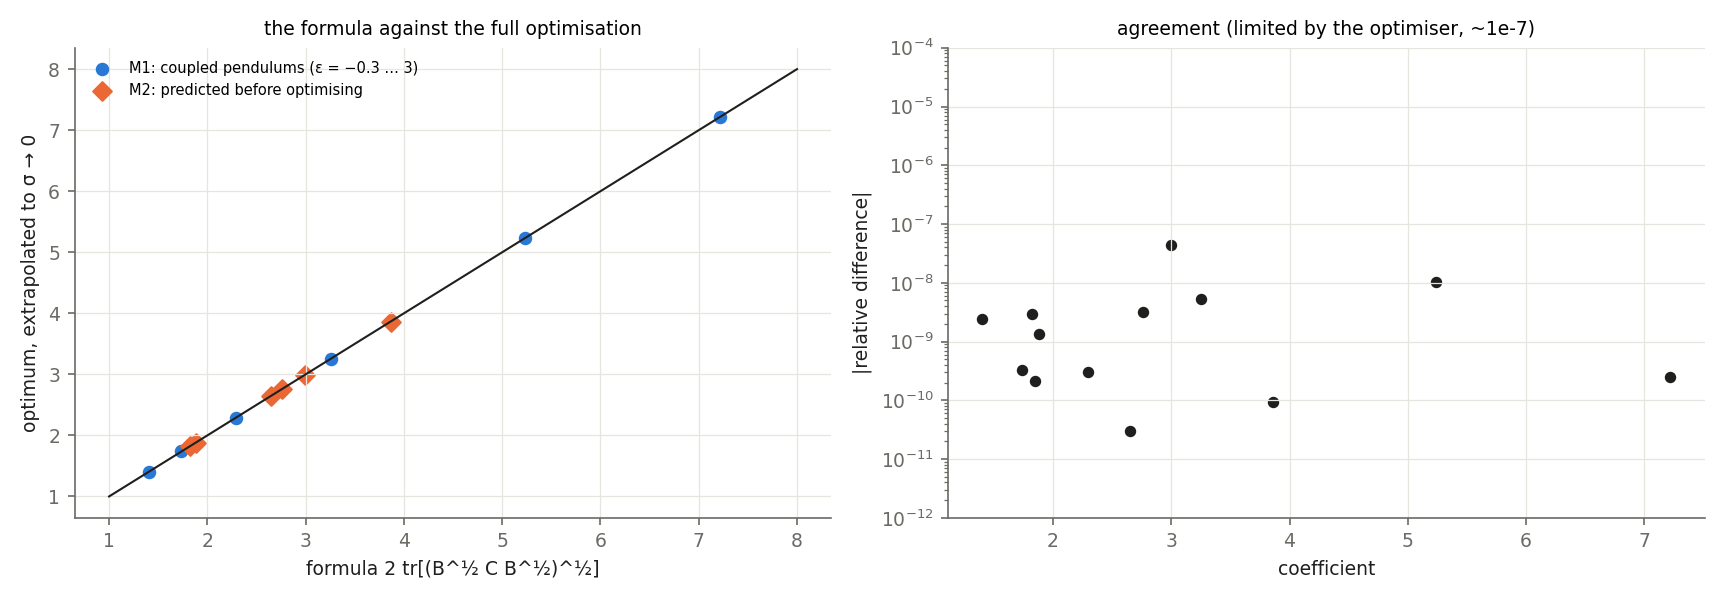
\includegraphics[width=0.95\textwidth]{figures/fig1_formula.png}
\caption{The formula $\Gamma = 2\tr[(B^{1/2}CB^{1/2})^{1/2}]$ against the best Gaussian state found by full optimization, extrapolated to $\sigma \to 0$. Circles: two coupled pendulums, $\varepsilon = -0.3$ to $3$ (Table~\ref{tab:coupled}). Diamonds: systems whose $\Gamma$ was recorded before the optimization (Sec.~\ref{sec:prediction}, Table~\ref{tab:prediction}). Right: relative difference, limited by the precision of the optimizer.}
\label{fig:formula}
\end{figure*}

\emph{The picture.} The observer's eye is a thin needle across the stretching direction of the first pendulum. It must be long in every other direction, but it pays only for the configuration directions on which the maximal strain depends: the contracting partner $w$ of the first pendulum, at the full price $2\kappa$, and the position of the second pendulum, at the price $\kappa$ weighted by the coupling. The second pendulum's momentum is free.
